%!TEX TS-program = xelatex
%!TEX encoding = UTF-8 Unicode
%!BIB program = biber

\documentclass[oneside, 11pt, letterpaper]{marl}

\proposaltitle{\doublespacing 
	Modern Generative Methods for Music Transcription
}

\threecommittee
{Professor Juan Pablo Bello, Chairperson}
{Professor Robert Rowe}
{Doctor Eric J. Humphrey}

\degree{Doctor of Philosophy}
\degreedate{\the\year}

\author{\href{mailto:jongwook@nyu.edu}{Jong Wook Kim}}
\program{Program in \href{http://steinhardt.nyu.edu/music/technology/}{Music Technology}}
\department{Department of \href{http://steinhardt.nyu.edu/music/}{Music and Performing Arts Professions}}
\university{\href{http://www.nyu.edu/}{New York University}}
\crest{}%\includegraphics[width=3in]{NYUlogoLarge2597}}
\submittedtext{Submitted in partial fulfillment\\
  of the requirements for the degree of\\
  Doctor of Philosophy in the\\
  \href{http://steinhardt.nyu.edu/}{Steinhardt School of Culture, Education, and Human Development}}

% turn of those nasty overfull and underfull hboxes
\hbadness=10000
\hfuzz=50pt
\makeindex

\addbibresource{library/library.bib}
\renewcommand{\doublespacing}{\setstretch{1.5}}

\begin{document}

\sloppy
\widowpenalty=10000
\clubpenalty=10000

%: ----------------------- generate cover page ------------------------
%\setstretch{1.2}
\maketitle  % command to print the title page with above variables
% \makecopyright

%: ----------------------- abstract ------------------------

% 
% Thesis Abstract -----------------------------------------------------


\begin{abstract}

\chapter*{Abstract}

{
\setstretch{1.3}
The problem of automatic music transcription (AMT) is considered by many researchers as the holy grail of the field, because of the notorious complexity and difficulty of the problem.
Meanwhile, the current decade has seen an unprecedented surge of deep learning where neural network methods have achieved tremendous success in many machine learning tasks including AMT.
The success of deep learning is largely enabled by the ever-increasing amount of available data and the innovation of GPU hardware, allowing a deep learning model to enjoy the increased capacity to process such scale of data.
While having more data and higher capacity translates better performance in general, there still remains the question of how to design an AMT model that effectively incorporates the inductive bias for the task and best utilize the increased capacity.

This thesis hypothesizes that an effective way to address this question is through the use of generative neural networks.
Starting with a simplified setup of monophonic transcription, we learn the effectiveness of convolutional representation and the roles of dataset choices in data-driven models for music analysis.
In the subsequent chapters, we examine the applications of deep generative models in music analysis and synthesis tasks, by introducing a WaveNet-based music synthesis model that learns a multi-dimensional timbre representation and a music language model applied in an adversarial manner to improve a piano transcription model.
Finally, we combine the analysis and synthesis methods and present a multi-instrument polyphonic music transcription system.
From these observations, we conclude that various forms of generative neural network can be used to provide better inductive bias to deep neural networks for automatic music transcription.


}

\end{abstract}


% ---------------------------------------------------------------------- 


%: ----------------------- tie in front matter ------------------------
\doublespacing
% % Thesis Dedictation ---------------------------------------------------

\begin{dedication} %this creates the heading for the dedication page

To Nayoung.

\end{dedication}

% ----------------------------------------------------------------------

% 
% this file is called up by thesis.tex
% content in this file will be fed into the main document

\chapter*{Acknowledgements}

I am truly grateful to many wonderful people who believed in me along this long journey. This dissertation would not have been able to come into existence without their support and guidance.

First of all, I would like to express my sincere gratitude to my supervisor, Prof. Juan Pablo Bello.
I am incredibly lucky to have you as my doctoral advisor; thank you for being a dependable teacher, an incredible researcher, and a welcoming friend to me.
To my committee members and readers --- Prof. Robert Rowe, Dr. Eric Humphrey, Prof. Johanna Devaney, and Prof. Brian McFee --- I deeply appreciate taking your time to read through my awkward sentences and giving insights to make them better.
And to all professors with whom I have had the pleasure of working with: thank you for your classes, chats, and smiles.

I have been fortunate enough to become friends with almost all of MARL's PhD students and postdocs, and I am thankful to every one of them.
To the MARL-doctors --- Taemin, Areti, Jon, Aron, Braxton, Finn, Eric, Uri, Rachel, and Finn --- thanks for showing the ways that I can follow, including but not limited to the coffee shops and bars.
To the MARL-doctor-to-be's --- Andrea, Andrew, Marta, Peter, Yu, Ho-Hsiang, Willie, Dirk, Tom, Jason, and Chris --- it was so much fun sharing office and hanging out with you, and I will miss the occasional beer sessions.
To the MARL postdocs --- Brian, Justin, Mark, Charlie, Ron, Vincent, Claire, Magdalena, Hitomi --- thank you for the insights during the lab meetings and collaborations, and also for sometimes bearing with my unscholarliness.

And to my Korean friends: thanks for being on KakaoTalk whenever I had silly memes to share with, but more importantly for being always welcoming and cheering for me every time I visited Korea, especially that time when you guys gladly spent a whole day at my wedding.

I am honored to have been a recipient of Samsung Scholarship, which is another factor that made all this possible; thank you for your support, networking, and gifts from Leeum.
I would also like to thank everyone I worked with during my brief industry experiences --- NCSOFT, Kakao, Pandora, and Spotify --- for allowing me to learn and achieve what I could not do in schools, and of course for all the free foods and swags.

To my parents who have always believed me and prayed for me, I can't express enough gratitude for your limitless love and unwavering support.
Your passion in education made me grow from an aspiring teenager to a respectable scientist.
Now that there are no more degrees for you to worry about, please take it easy and enjoy your 60s!

Finally, to my wife Nayoung, you are the foremost reason why I am writing these words now.
I cannot believe how lucky I am to have met you and plowed through this journey mixed with joys and tears with you.
Thank you for being my best friend, a fellow researcher, a delightful travel partner, a world-class cook, a witty comedian, and a lovely cheerleader who makes me a better person every day.



\singlespacing

%: ----------------------- contents ------------------------
% levels are: 0 - chapter, 1 - section, 2 - subsection, 3 - subsubsection
\setcounter{secnumdepth}{3} % organisational level that receives a numbers (NYU Steinhardt recommends level 0, which is pretty hideous)
\setcounter{tocdepth}{2}    % print table of contents for level 2

{
	\small 
	\tableofcontents            % print the table of contents
	%\addcontentsline{toc}{section}{continued}
	%: ----------------------- list of figures/tables ------------------------
	
	%\clearpage
	%\listoftables                   % print list of tables
	\clearpage
	\listoffigures                  % print list of figures
}

%: ----------------------- glossary ------------------------

% Tie in external source file for definitions: /frontmatter/glossary.tex
% Glossar entries can also be defined in the main text. See glossary.tex

%\include{frontmatter/glossary}
%\makeglossaries
%\clearpage
%\printglossaries

\chapterbegin

%: ----------------------- epigraph ------------------------
% 
\chapter*{}

\begin{quote}
``What I cannot create, I do not understand.''

\end{quote}

\vspace{1in}
\hspace{2in}
-Richard Phillips Feynman 

%: --------------------------------------------------------------
%:                  MAIN DOCUMENT SECTION
% --------------------------------------------------------------

% the main text starts here with the introduction, 1st chapter,...

\mainmatter
\doublespacing

%: ----------------------- subdocuments ------------------------

% Parts of the thesis are included below. Rename the files as required.
% But take care that the paths match. You can also change the order of appearance by moving the include commands.

%!TEX root = ../dissertation.tex
% this file is called up by thesis.tex
% content in this file will be fed into the main document

%: ----------------------- introduction file header -----------------------
% the code below specifies where the figures are stored
\graphicspath{{1-introduction/figures/}}

\chapter{Introduction}
\label{ch:introduction}

As listening is a core constituent of human perception, an essential component of artificial intelligence is \emph{machine listening}.
The purpose of machine listening research is to enable computers to process and understand sounds as humans do.
In recent years, there have been an unprecedented amount of successes in the field of \emph{machine learning}, a near-synonym to artificial intelligence with a connotation of statistical and/or probabilistic methodologies, which redefined what a computer vision or natural language processing systems can do and made previously unimaginable applications such as autonomous driving and a superhuman Go-playing AI into reality.

In this context, this thesis focuses on improving the machine understanding of music in order to automatically transcribe music, which largely remains an unsolved problem despite decades of research.
The recent rapid development in \emph{deep learning} research, however, hints at many new possibilities for improving the performance or even achieving human-level accuracy in music transcription.

\section{Statement of Problem}\label{sec:statement}

\begin{figure}
	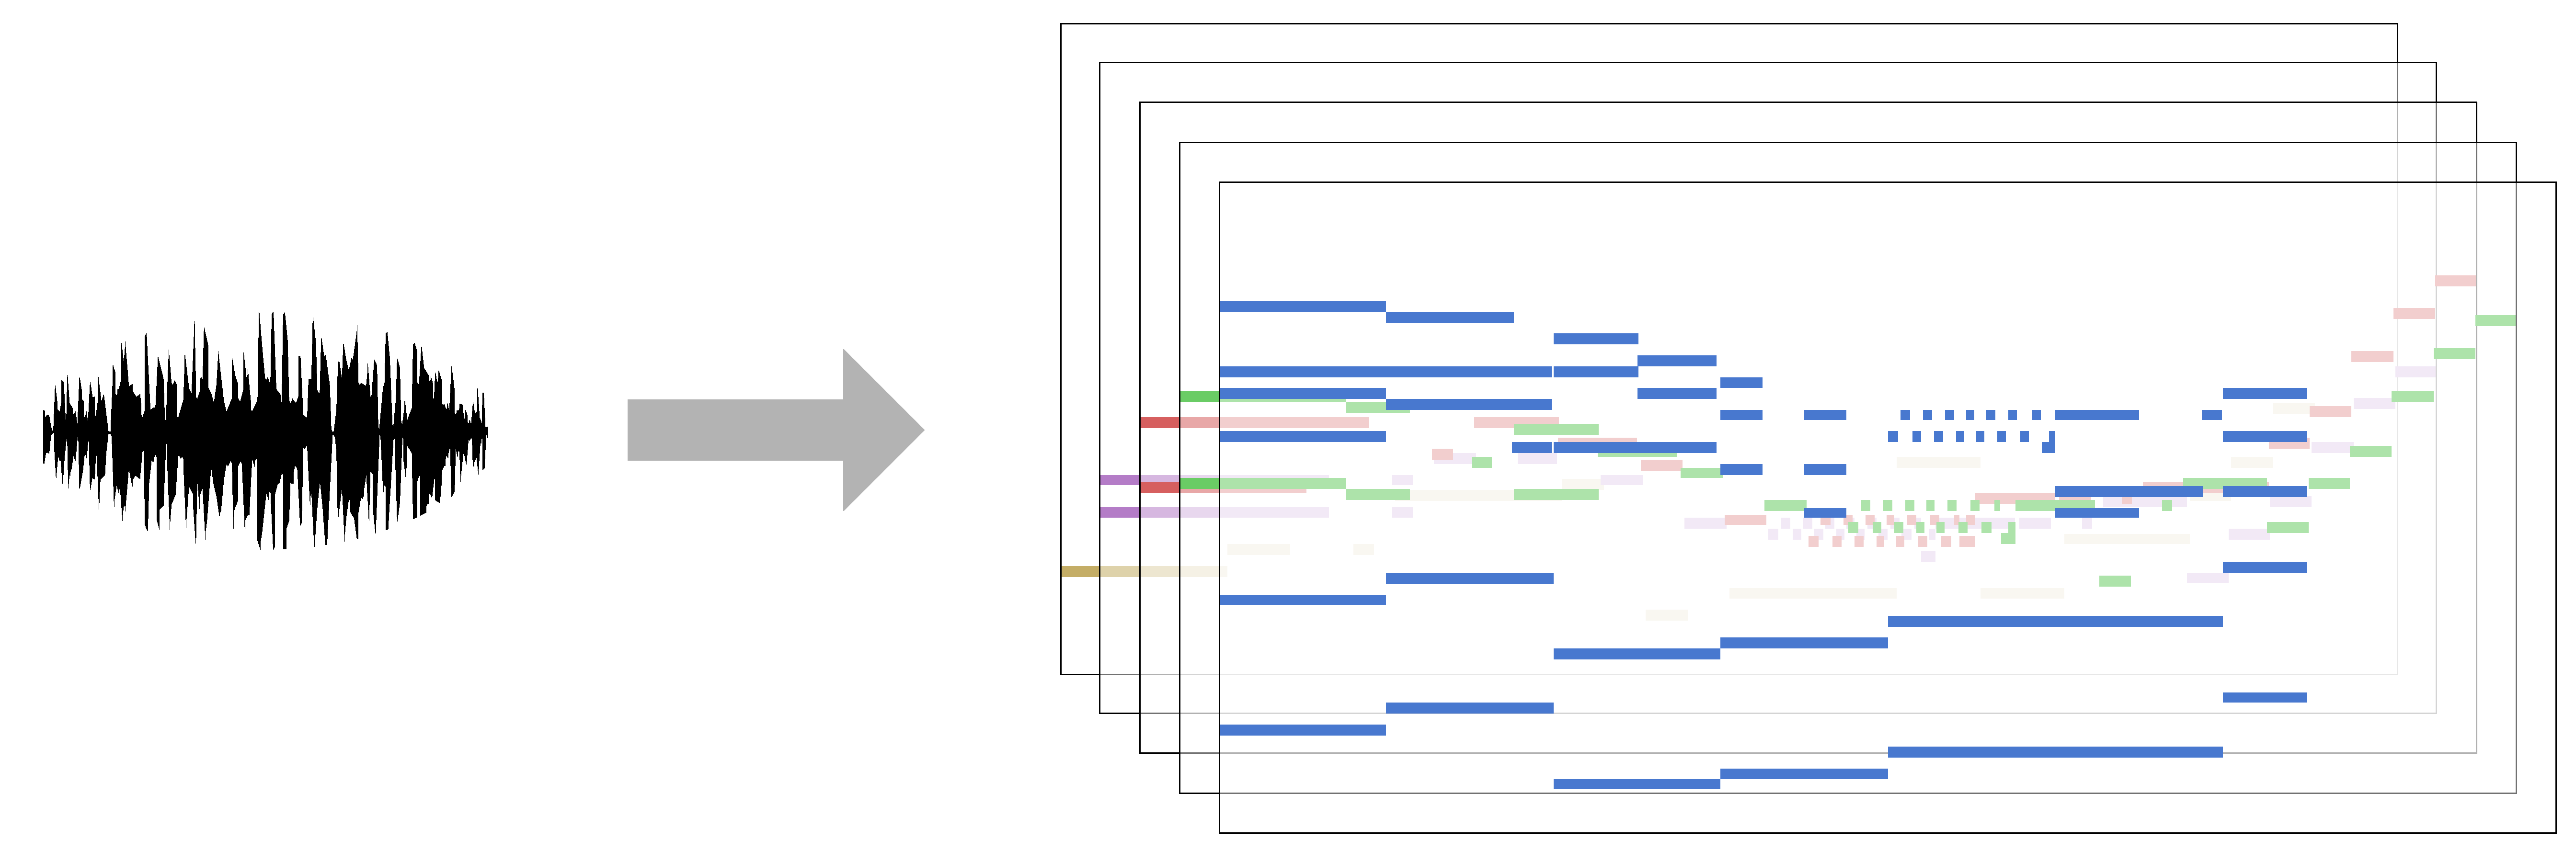
\includegraphics[width=\textwidth]{march-transcription.pdf}
	\caption{The automatic music transcription setup to be used in this thesis. Using per-instrument piano-roll representations is easier for machines to process, and avoids variability and subjectivity that may arise from symbolic and textual notations.} 
	\label{fig:transcription-to-piano-rolls}
\end{figure}

\emph{Automatic music transcription} (AMT) refers to an automated process that can identify musical events in the input audio and convert them into musical notations.
Historically, the definition of automatic music transcription varied by author, usually in terms of the form of the output representation.
In earlier works \cite{moorer1977transcription,piszczalski1977transcription}, the final output of the transcription system was to be the common music notation, i.e. a score, while later literature generalizes the problem by defining it as ``the analysis of an acoustic musical signal so as to write down the pitch, onset time, duration, and source of each sound that occurs in it" \cite{klapuri2006transcription} or ``the process of converting an acoustic musical signal into some form of musical notation" \cite{benetos2013amt}.
This thesis adopts per-instrument piano-rolls as the resulting representation of automatic music transcription, as shown in Figure \ref{fig:transcription-to-piano-rolls}, and defers the ``piano-roll to score" conversion as an out-of-scope task, which involves higher-level nontrivial tasks such as tempo and meter tracking, key signature detection, and music structure identification.
This can be justified since it allows the transcription model to focus on source separation and multi-pitch tracking, which are already highly challenging problems \cite{cemgil2006generative}.


To perform automatic music transcription, various properties of musical events, such as pitch, timbre, harmony, beats, etc., need to be defined and extracted from the audio.
In this sense, the setup of AMT is \emph{discriminative} in nature, meaning that it aims to identify different attributes from given audio, as opposed to \emph{generative} models concerning how to construct audio signals according to given conditions about those attributes.
Meanwhile, when a generative model is jointly trained with an encoder, it can learn to generate data samples from a small number of latent factors, while the encoder learns to extract those factors from the audio in a compact representation, as depicted in Figure \ref{fig:autoencoder}.
Since recently, with the increased capacity of machine learning models and hardware, many \emph{deep generative models} have been proposed and shown to be capable of processing high-dimensional multimedia data.
Furthermore, significant research efforts have been made toward learning disentangled representation of data, meaning that the latent factors contain meaningful information that can be easily separated and isolated.
To this end, the goal of this thesis is to study representation learning methods powered by deep generative models, accompanied with automatic generation of music, to obtain disentangled information from audio signals that can achieve better performance in music transcription.

\begin{figure}[t]
	\includegraphics[width=\textwidth]{autoencoder.pdf}
	\caption{A generative model has to know all of necessary information required to reconstruct the audio data, including pitch, timbre, loudness, and duration. Generative models can be jointly trained with an encoder that finds those semantic information, giving a transcriber-synthesizer pair; more detail on Subsection \ref{ch:deeplearning}.\ref{subsec:gan-encoder}.}
	\label{fig:autoencoder}
\end{figure}

\pagebreak

\section{Subproblems and Research Questions}\label{sec:subproblems}

This thesis concerns two major subproblems regarding the proposed approach toward automatic music transcription: 

\vspace{1em}

\begin{enumerate}
	\item Can we use generative methods to obtain disentangled representations of musical audio signals, to be used for automatic music transcription?
	\begin{enumerate}
		\item Can deep generative models such as \emph{generative adversarial networks} (GAN) learn to differentiate the concept of pitch and timbre, so that it can separately control them in its generation?
		\item How can we extend such generative model to work with arbitrary time scales, learning to encode and generate polyphonic notes with various onset times and durations?
		\item Can we make the latent representation used in the generative model convey information on the note-level events in the form of piano rolls, effectively performing music transcription?
	\end{enumerate}
	\item Can we build a music generation pipeline as a data augmentation tool which provides a large-scale representative dataset for training, in order to more effectively train the transcription model?
	\begin{enumerate}
		\item Can we use software instruments and audio post-processing techniques to span various timbres and recording environments that we are expected to encounter in transcription?
		\item How can we formulate a music language model that can be plugged into music synthesis and build generalizable datasets for polyphonic, multi-instrument music transcription?
		\item Would it be possible to incorporate the music generation pipeline into the deep generative model as a learnable component of the automatic music transcription algorithm?
	\end{enumerate}
\end{enumerate}

\vspace{1em}

The primary objective of this thesis lies on the first subproblem, concerning the disentanglement in representation learning on musical audio powerd by deep generative models.
Necessary to the successful application of data-driven learning is the availability of large-scale training data, while the difficulty of obtaining large-scale labeled data has always been a problem in music informatics.
The second subproblem is aimed at alleviating this issue by employing automatically generated datasets using software instruments and music language models.
In this sense, while not being the primary research objective of the thesis, effectively designing the data generation pipeline would be an indispensable component of achieving the primary goal.

\section{Definitions}\label{sec:definitions}

\paragraph{Research Areas}

\begin{itemize}
	\item \textbf{Music Information Retrieval (MIR)}: An interdisciplinary research area that concerns retrieving information from music.
	\item \textbf{Automatic Music Transcription}: An automated process of extracting musical events in the input audio and converting them into musical notations.
	\item \textbf{Multi-Pitch Estimation}: A task of estimating individual pitch values in polyphonic music. Synonymous with \textbf{Multiple Fundamental Frequency (F0) Estimation}.
\end{itemize}

\noindent 
\paragraph{Music and Audio Signal Processing}

\begin{itemize}
	\item \textbf{Pitch}: A perceived quality of highness or lowness of a sound that is closely related to the fundamental frequency.
	\item \textbf{Spectrogram}: A two-dimensional representation of an audio signal that visualizes the spectral decomposition of the sound over time, using the magnitudes of the short-time Fourier transform (STFT).
	\item \textbf{Short-Time Fourier Transform (STFT)}: A linear transformation that maps a one-dimensional signal to a two-dimensional representation that contains the Fourier spectra of the short-time segments.
	\item \textbf{Music Language Model}: Modeling of symbolic sequences of music.
\end{itemize}

\paragraph{Machine Learning and Deep Learning}

\begin{itemize}
	\item \textbf{Heuristics}: A method that is not optimal or perfect but useful for immediate practical purposes, usually employing manually designed functions or computations.
	\item \textbf{Data-Driven Method}: A method based on the optimization of model parameters using examples of data.
	\item \textbf{Ground-Truth}: Annotations corresponding to the data examples that are assumed to be true.
	\item \textbf{Machine Learning}: Programming computers to learn from experience, without being explicitly programmed \cite{samuel1959ml}.
	\item \textbf{Supervised Learning}: A category of machine learning methods that require labeled training data.
	\item \textbf{Unsupervised Learning}: A machine learning task to discover the hidden structures from unlabeled data.
	\item \textbf{Deep Learning}: A family of machine learning methods that employ multiple layers of learned representations, obtained by composing simple transformations at each level \cite{lecun2015deeplearning}.
	\item \textbf{Representation Learning}: A task of learning the underlying representations of data that make it easier to extract useful information \cite{bengio2013representation}.
	\item \textbf{Generative Model}: A model that is capable of generating data points that are coherent to supplied training examples.
	\item \textbf{Disentanglement}: A desirable quality of a learned representation from which meaningful information can be easily separated and isolated.
\end{itemize}

\section{Delimitations/Limitations}\label{sec:limitations}

Because of the sophisticated and open-ended nature of automatic music transcription, it is necessary to define the scope of the tasks and data that this thesis will be concerned with.
The purpose of this section is to define those limitations in terms of the scope of music that the proposed AMT system can process, the required capability of symbolic music processing, and the need for the perceptual studies regarding the validity of AMT systems.


\subsection{Scope of Music}

Music signals typically contain both harmonic and percussive sources. 
In the signal processing point of view, harmonic sounds are periodic and contains energy only at certain frequencies usually at the multiples of the fundamental frequencies, whereas percussive sounds have continuous frequency spectra in which it is not possible to define a fundamental frequency.
Consequently, transcription models for harmonic sounds and percussive sounds require different techniques according to their nature.


This thesis will limit the focus on the transcription of harmonic sounds and therefore use the per-instrument piano roll notation (Figure \ref{fig:transcription-to-piano-rolls}) as the output representation.
This is a realistic trade-off to make, because of a number of reasons.
First, learning to simultaneously model the harmonic and percussive sounds is a harder problem both conceptually and computationally.
Secondly, it is possible to plug a harmonic-only model into a pipeline consisting of HPSS (harmonic-percussive source separation) and a percussion transcription model as an alternative to the comprehensive approach.
Lastly, polyphonic transcription is considered to be the most difficult problem in the domain of automatic transcription, and it is sensible to tackle this as a standalone problem in a simplest possible setup.
Excluding percussive sounds will disallow using most of pop music tracks as-is, but multi-track datasets can still be utilized since they contain each track separately.


Additional limitations should be considered on the types of the instruments and their sound variations.
Depending on the instrument, the same line segment in a piano roll representation may contain a variety of musical techniques, such as vibrato, tremolo, pizzicato, and the usage of a mute or harmonics, among others.
In order to accurately produce the piano roll transcription that is invariant to those variations, the model has to be trained to classify them as nonessential information, requiring the availability of the dataset with the annotations for those techniques.
While an ideal model should learn those concepts as humans do, too much timbral or temporal variation for an instrument will prevent the model from learning a consistent representation corresponding to the instrument.
Therefore, for the immediate purpose of this thesis, a dataset that does not contain too much variations will be employed, similarly to the pilot study which used non-vocal harmonic sounds of Western classical instruments.


\subsection{Symbolic Processing of Notes}

As mentioned and justified in the statement of problem (Section \ref{sec:statement}), by choosing per-instrument piano rolls as the output of transcription, many structure-level and symbolic-level concerns in music transcription are excluded from the scope of this study.
The difference between the piano roll output and the full human-readable score output becomes apparent when we compare the piano rolls in Figure \ref{fig:transcription-to-piano-rolls} with Figure \ref{fig:wedding-march-score}, which is the original score from which the piano rolls are plotted.
There are many aspects in producing the score output that are highly subjective and difficult to derive a consistent evaluation metric from, such as the interpretation of legatos or staccatos and the aesthetic choices for typesetting, providing an additional justification for using the piano roll notation.


The MIDI file format is suitable for conveying the data equivalent to per-instrument piano rolls, consisting of multiple tracks of \texttt{note\_on} and \texttt{note\_off} events with the corresponding timestamps.
MIDI will therefore be the output format of the proposed AMT system, which can also be conveniently played back by media player software.
Music typesetting software such as Sibelius or Finale can render a MIDI file into a score notation using the metadata in the file as well as some heuristics for quantization, however the readability of the score rendered from a transcribed MIDI file would be limited, due to imperfect transcription and the absence of metadata on the time and key signature.


\begin{figure}
	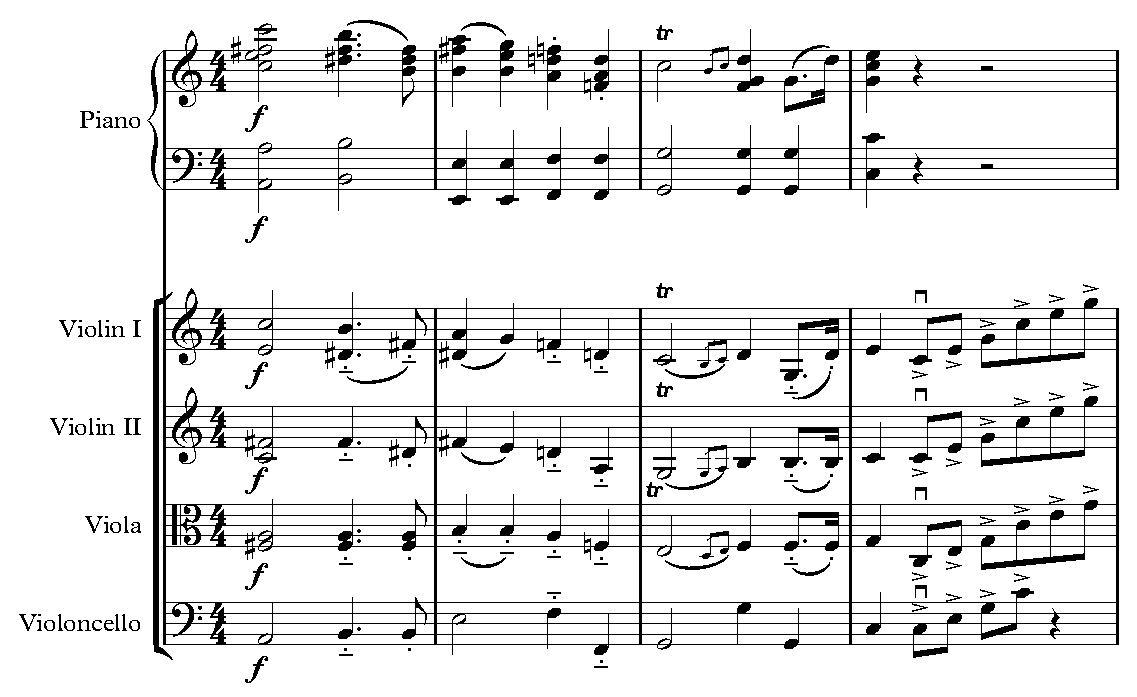
\includegraphics[width=\textwidth]{march-score.pdf}
	\caption{The full score notation of the music used to build the piano rolls in Figure \ref{fig:transcription-to-piano-rolls}. To fully recover this level of notations from the audio, the transcriber has to make many additional decisions than for the piano rolls, such as determining the key signature, time signature, clefs, dynamics, trills, bowing instructions, etc.}\label{fig:wedding-march-score}
\end{figure}



\subsection{On the Need for Perceptual Studies}

This study of automatic music transcription is entirely quantitative and does not involve subjective tests on human participants.
The dataset to be used in thesis consists of audio signals, i.e. waveforms encoding the physical vibrations of air.
However, music is essentially a perceived notion, and thus are the core qualities of sound --- pitch, timbre, and loudness --- which are the output of automatic transcription.
For this reason, manually annotating polyphonic music is an error-prone process, where any two annotators may produce drastically different annotations.
Although this problem of inaccuracy and subjective difference is often overcome by using a ground-truth dataset synthesized from known frequency information, the gap still persists between what a model can learn from synthesized audio and what it will respond to the real-world sound.
This thesis aims to take one step further than using synthesized training datasets, by building a generative model that can better model the real-world sound of interest.

The goal of automatic transcription is at a lower level than the tasks like chord recognition and melody tracking, which may incur even more subjective disagreements caused by the imprecise definitions of chords and melodies.
Pitch is relatively precisely defined in this sense, and formulating automatic music transcription as an audio-to-piano-roll conversion mostly eliminates the ambiguity that exists in chord recognition and melody tracking.
There exist some cases where the mathematical definition of fundamental frequency still cannot be applied for all pitched sounds, such as the Shepard tone \cite{shepard1964circularity} where the pitch of a harmonic sound fails to be consistently mapped to a fundamental frequency.
However, disregarding these few edge cases, this study assumes that the piano roll notation can convey an objective transcription for practical purposes, postulating AMT as a mathematical problem which does not require experiments on human subjects.


\subsection{The Ultimate Goal of Automatic Music Transcription}

Finally, a consideration is needed for the fundamental limitation on any music transcription task, either automatic or manual, and when it can be said that AMT is solved.
Polyphonic music contains a mixture of sounds with an indefinite number of notes being played simultaneously; even the most experienced musicians may not be able to identify every note, and the audio mixture may not contain the sufficient information to convey all notes in the first place.
It would be unreasonable to expect anyone to perfectly transcribe all notes in the score of an orchestral music from an audio file, but it would be sensible for a trained musician to produce a version of score that, when played by the same orchestra, sounds indistinguishable to the original recording.
Considering these limitations, passing this ``transcriptional Turing test'' as shown in Figure \ref{fig:turing}, rather than achieving the 100\% accuracy on a certain dataset, should be the ultimate goal of automatic music transcription, at which point it can be said to have a human-level intelligence on this task.

Developing an AMT algorithm that can pass this test is not a goal of this thesis, because the performance of AMT is far behind the human performance.
Therfore, this thesis pursues a more tangible goal of achieving a better accuracy in transcribing music that is easy enough for human transcribers but challenging for machines.
More details on the dataset and the evaluation method are provided in Chapter \ref{ch:methods}. \TODO{FIX}


\begin{figure}
	\includegraphics[width=\textwidth]{turing.pdf}
	\caption{The \emph{transcriptional Turing test}, to test whether an automatic music transcription algorithm has reached human-level. While this provides some conceptual insights to the adversarial training setup, to be covered in the later chapters, fully achieving the human-level performance is out of scope of this thesis.}
	\label{fig:turing}
\end{figure}

\pagebreak

\section{Need for Study}

The nature of music transcription is multifold; to create a complete transcription, one has to identify all instruments, onsets, dynamics, and the pitch traces for every instrument present in the music, and it is still far from achieving the human-level accuracy.
The need for study arises naturally, not only because this is an intriguing problem in the interdiscipline of music and technology that has remained unsolved for decades, but also because the solution to this problem can provide practical benefits to many applications.

In order to bolster the need for this study, this section starts by introducing such applications, followed by discussions on the advantages of employing generative models as a means of better capturing musical semantics and a new paradigm of MIR research.
A brief perspective on AMT is presented in the context of wider AI research, followed by the organization of the chapters.


\subsection{Applications of Automatic Music Transcription}\label{sec:applications}

Many applications of the techniques in the realm of automatic music transcription is on interactive music systems.
\citeA{vercoe1984performer} proposed a quest for a \emph{synthetic performer}, which can listen, perform, and learn in the context of live performance, and automatic \emph{real-time accompaniment} \cite{dannenberg1985accompaniment} based on dynamic programming was one of the first successful demonstrations of AMT techniques.
\emph{Score following} is a general term referring to the synchronization of a computer with a performer playing a known score \cite{orio2003following}.
An offline music-to-score matching algorithm can also be applied to intelligent audio editors \cite{dannenberg2003following}.

Music recommender systems can combine many kinds of information for improved music retrieval and personalization \cite{celma2010music}.
Content-based music recommender systems can utilize not only the metadata but also the audio content, and methods using timbral \cite{magno2008recommendation}, temporal \cite{li2007recommender}, and tonal features \cite{lu2009recommendation} have been introduced.
These music recommender systems can be further improved when the complete information on each domain is made available through AMT.

AMT system can help create the database for query-by-humming \cite{ghias1995humming} by automatically creating melody annotations, where users can retrieve music by humming an excerpt of the song.
Such database can also facilitate a large-scale musicological analysis \cite{abdallah2015british}, as well as the development of computer-aid music composition \cite{agostini2013aid} that incorporates musicological knowledge.


\subsection{Generative Modeling for Fully Capturing Semantics}

Being ``generative'' means that a model is capable of generating new samples in the domain of the original data.
Generation in the symbolic domain creates new musical scores, and a generative model in the audio domain creates audio waveform.
These two kinds of generative systems are familiar to computer music artists and are referred to as algorithmic composition \cite{fernandez2013ai} and sound synthesis \cite{cook2002synthesis} models.
This thesis defines the term ``generative model'' more specifically, as a model that can learn the distribution of provided data and can sample new samples in the original distribution.
This differs from the term ``generative'' used in computer music in a sense that it aims to accurately model and learn to regenerate the real-world audio to be used in music transcription, rather than focusing on artistic aspects of generating new kinds of sounds and music.

By learning to generate data using fewer parameters than the scale of the dataset, a model has to discover the underlying natural features from the distribution of data.
In music transcription, these features correspond to the musical concepts such as pitch, timbre, and rhythm.
This idea follows what Richard Feynman once wrote on his blackboard, \emph{``What I cannot create, I do not understand''} and \emph{``Know how to solve every problem that has been solved''}.
He meant that the marker for truly understanding something is the ability to construct it completely from scratch.
Generative models are a branch of unsupervised learning, because it does not require labeled data.
\citeA{lecun2016unsupervised} introduced unsupervised learning as a cake, comparing supervised learning as icing and reinforcement learning as the cherry on the top, by which he meant that generative model needs to predict much larger scale of information but is able to learn the ``common sense''.

\begin{figure}
	\includegraphics[width=\textwidth]{generative-evolution.pdf}
	\caption{Increasingly realistic qualities of the generated faces using generative adversarial networks as shown in \protect\cite{brundage2018malicious}; images are from \protect\cite{goodfellow2014gan}, \protect\cite{radford2015dcgan}, \protect\cite{liu2016cogan}, and \protect\cite{karras2017pggan}.}
	\label{fig:generative-evolution}
\end{figure}


Inherently, unsupervised learning is less well-defined than supervised learning, and this is the reason why unsupervised learning is sometimes synonymous with clustering, because finding clusters is usually as much an unsupervised learning system can do.
However, a recent success of deep learning introduced a new breed of generative models, enabling an end-to-end generation of complex data such as photos and audio signals.
\emph{Generative adversarial network} (GAN) \cite{goodfellow2014gan} is the most notable among them, and its performance in generating realistic images has been improving at an extraordinary pace, as shown in Figure \ref{fig:generative-evolution}.
Combined with the various techniques for manipulating the semantic information in GANs as will be introduced in Section \ref{ch:deeplearning}.\ref{sec:gan}, this hints at a completely new kinds of generative methodologies for audio processing.


In this context, this thesis aims to design and develop improved methods for automatic music transcription with a deeper understanding of musical semantics powered by deep generative models.
The idea specifically hypothesizes that by training a generative model, it is possible to learn disentangled representations, from which the information necessary for transcription can be easily extracted, as depicted in Figure \ref{fig:autoencoder}.
By doing so, the ultimate objective is to build an end-to-end differentiable model that connects the piano roll representation to audio signals, in order to perform automatic music transcription --- obtaining the most likely piano roll representation for given audio.


\subsection{Generative Models as a new Paradigm of MIR Research}

\begin{figure}
	\begin{subfigure}[b]{\textwidth}
		\centering
		
\includegraphics[width=0.75\textwidth]{paradigms-1-manual.pdf}
		\caption{A traditional rule-based model based on hand-crafted features.}
		\label{}
	\end{subfigure}
	\begin{subfigure}[b]{\textwidth}
		\centering
		\vspace{1em}
		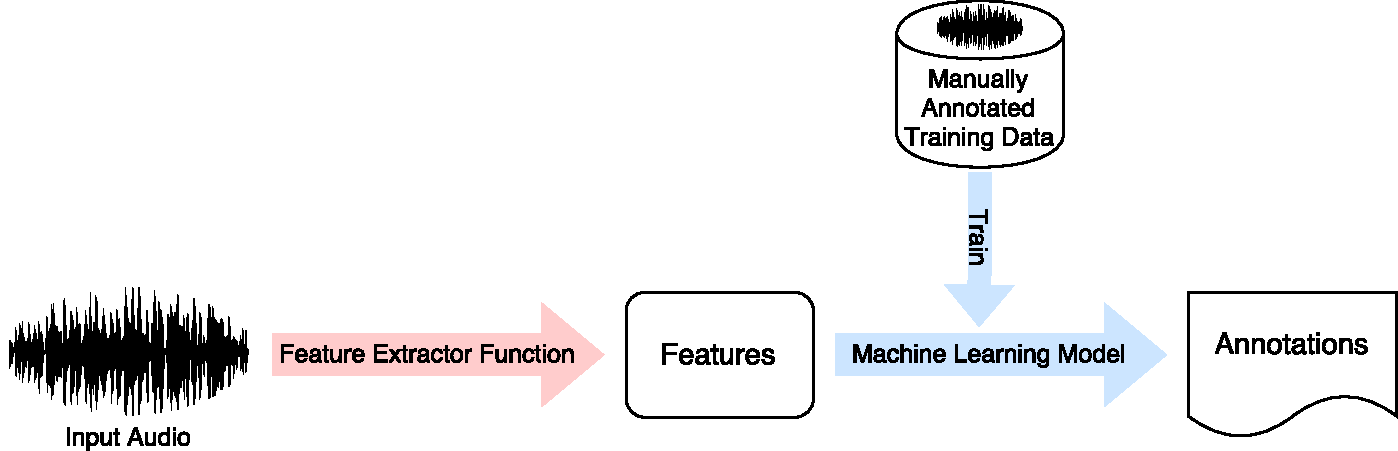
\includegraphics[width=0.75\textwidth]{paradigms-2-features.pdf}
		\caption{A data-driven machine learning model built upon hand-crafted features.}
		\label{}
	\end{subfigure}
	\begin{subfigure}[b]{\textwidth}
		\centering
		\vspace{1em}
		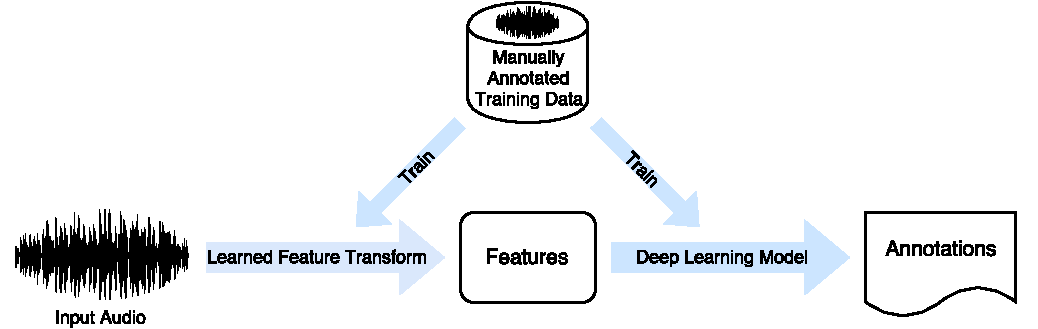
\includegraphics[width=0.75\textwidth]{paradigms-3-end-to-end.pdf}
		\caption{An end-to-end data-driven model without manual feature engineering.}
		\label{}
	\end{subfigure}
	\begin{subfigure}[b]{\textwidth}
		\centering
		\vspace{1em}
		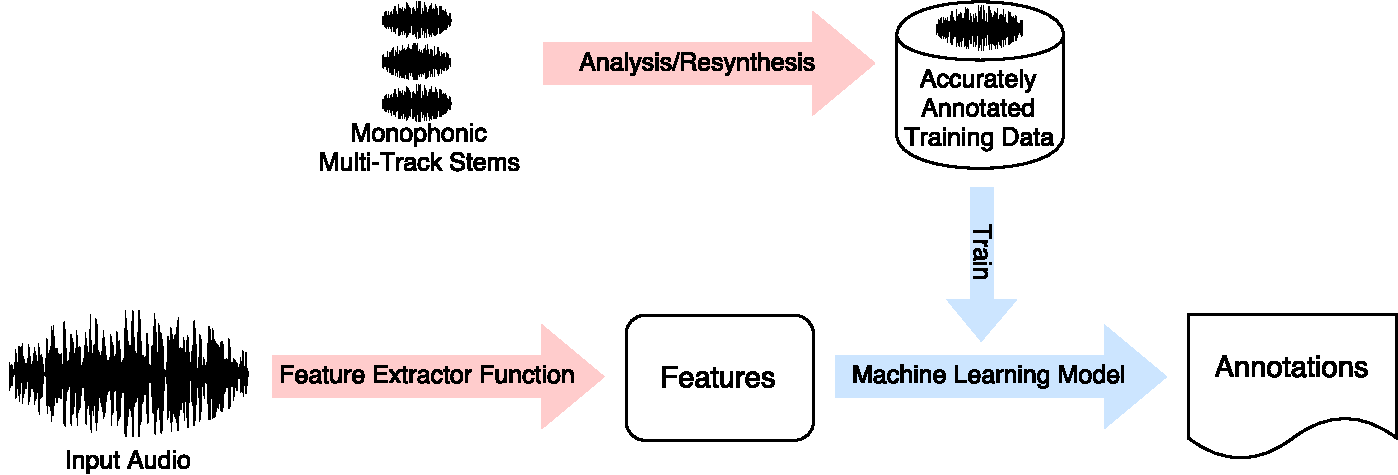
\includegraphics[width=0.75\textwidth]{paradigms-4-analysis-synthesis.pdf}
		\caption{Analysis/synthesis \cite{salamon2017analysis} for accurate and automatic annotation.}
		\label{}
	\end{subfigure}
	\begin{subfigure}[b]{\textwidth}
		\centering
		\vspace{1em}
		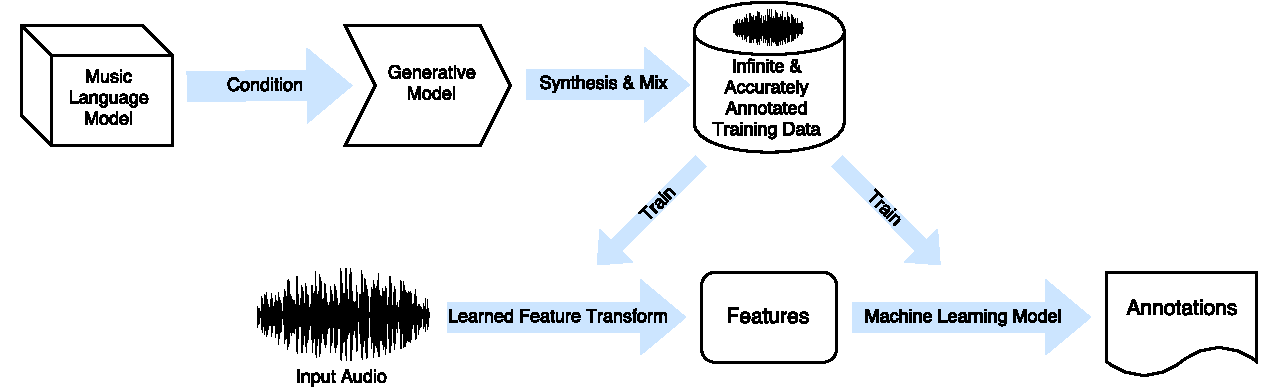
\includegraphics[width=0.9\textwidth]{paradigms-5-proposed.pdf}
		\caption{The proposed setup, leveraging the music language model and the generative model providing an infinite source of accurately annotated training data.}
		\label{}
	\end{subfigure}
	\caption{Paradigms of MIR research. Blue arrows indicate learnable components.}
	\label{fig:paradigms}
\end{figure}


The second subproblem stated in Section \ref{sec:subproblems} considers data generation as an augmentation tool for further improving the performance of an AMT system.
In the proposed setup, a music language model is trained to produce meaningful symbolic music sequences to be fed to the generative model, which can synthesize multi-track polyphonic music along with the corresponding annotations.

This architecture can be aligned with the previous paradigms of MIR research, as shown in Figure \ref{fig:paradigms}:
(a) The earlier methods typically use a carefully crafted function to extract features and performed rule-based predictions, whereas (b) the data-driven methods replace the later part with a machine learning model trainable with a dataset.
(c) With the access to a larger amount of data and deep learning techniques, end-to-end models eliminate the need for manually designed feature extractors by learning the feature transform directly from data.
(d) The analysis/synthesis model \cite{salamon2017analysis} overcomes the data scarcity problem by automatically generating annotations from multi-track stems, to be supplied to a polyphonic transcription model.
A shortcoming of this approach is that it requires a multi-track dataset composed of monophonic stems.
(e) The proposed setup extends the analysis/synthesis model by building a fully learnable pipeline, where the synthesizer component of the generative model serves as an effectively infinite source of labeled training examples.

In theory, this can constitute a positive feedback loop where data augmentation improves the performance of the transcription model, and the improved synthesizer component of the transcription model provides better data augmentation.
Another advantage of this setup is that the data augmentation pipeline is not limited to training an AMT model but applicable to any music information retrieval tasks.

\subsection{In the Broader Context of Machine Listing in AI Research}

Using generated audio data and generative models is partly motivated by the fact that synthesized music is more prevalent and perceptually more familiar to people than synthesized texts or pictures, considering that many commercial music tracks are often produced entirely using software instruments, except for the vocal parts.
This suggests that synthesized and generated audio may more accurately model the distribution of the real audio data to be transcribed.
This generative approach also aligns well with how actual musicians transcribe music, where they match given audio with their knowledge of how the instruments sound when played in a certain combination of rhythms and melodies.
Therefore it is reasonable to claim that machines should also be able to perform in a similar way, provided that a proper representation of knowledge about the music and instruments is available.

The task of automatic music transcription shares many common values with other machine learning tasks, such as image segmentation, machine translation, and speech recognition, in a sense that the core task is to build an intelligent system that can extract and process semantics that are conveyed in complex signals.
This is an essence of artificial intelligence (AI)
--- a system that perceives its environment and takes actions that maximizes the utility \cite{russell2009ai} --- 
where an intelligent system has to understand the semantics of complex data coming from the environment in order to perform well in its tasks.
To this end, the problem of automatic music transcription is not just an intriguing task in music technology, but will also be a key component of the AI-enabled future society, constituting a musical brain of AI in the form of advanced machine musicianship \cite{rowe2003musicianship}.


\subsection{Organization of Thesis}


To summarize, this thesis considers the possibility of using deep generative models to learn the musical concepts necessary for automatic music transcription, as well as using the learned generative component as an augmentation tool for further improving the performance of the transcription model.

There exists a rich history of research aiming at understanding of musical sounds and automatic music transcription, and to validate this claim as a feasible research direction and place this proposal in the context of this continuum of research, Chapter \ref{ch:mir} provides a review of the standard methods and the current state of the art of automatic music transcription research.
%One of the most exciting phenomena that have been happening in the field of machine learning during the past five years is the advent of deep learning and its tremendous success in computer vision, natural language processing, and many other fields.
%The success was made possible by the unprecedented scale of high-performance computing resources that became available, which made intelligent systems capable of processing machine learning algorithms and data pipelines that were infeasible to be realized just until a few years ago.
%At the same time, a number of new models and techniques have been devised to drastically improve the effectiveness and flexibility of existing algorithms.
Because it is expected that the techniques of deep learning will play the most important role in this study, a general introduction to deep learning and deep generative models is provided in Chapter \ref{ch:deeplearning}, with a focus on generative adversarial networks, which are by far the most capable family of deep generative models.


Chapter \ref{ch:methods} presents the tentative design of the proposed automatic music transcription research, along with the architecture of the deep generative model and the datasets to be used.
%The pipeline incorporates deep learning and music signal processing methods as well as other important components including data augmentation, software instruments, audio synthesis, and music language models.
Subsequently, some results of the preliminary experiments in this direction of research are introduced in Section \ref{ch:pilot}, including a monotonic pitch estimator based on time-domain convolutional neural network and a generative adversarial network trained on log-magnitude spectrograms of instrument note samples.
%!TEX root = ../dissertation.tex
% this file is called up by thesis.tex
% content in this file will be fed into the main document

%: ----------------------- introduction file header -----------------------
% the code below specifies where the figures are stored
\graphicspath{{2-deeplearning/figures/}}

\chapter{Deep Learning in a Nutshell}\label{sec:deeplearning}
\label{ch:deeplearning}

Since recently, a family of machine learning research under the buzzword "deep learning" has incurred groundbreaking changes to the world of artificial intelligence, making the long-waited dream of the strong artificial intelligence look not so distant in the future.
The impact of deep learning was so dramatic that many successful applications of deep learning like DeepMind's AlphaGo beating the human Go champion and Google's neural machine translation have became familiar to laypeople.
The core idea of using artificial neural network to process complex information traces back to the very early days of computing \cite{kleene1951representation}, but it has long been considered less effective than alternative methods, such as support vector machines or probabilistic graphical models.
Around 2010, it turned out that neural networks can substantially outperform those other approaches and have much more flexibility for the further improvements, and the lower performance of neural network was simply due to the insufficient data, the lack of computational power, and some tricks that have not been employed before.
This finding has opened the era of deep learning, a term coined after the fact that neural networks often employ multiple layers of learned feature transformations, and is continuing to innovate virtually all fields of science and engineering, including, of course, music technology.

Because it is expected that the methodologies and techniques of deep learning will play a crucial role in the thesis, this chapter briefly covers the essential concepts and terminologies of deep learning. Starting from the basic architectures and techniques, more emphasis will be given on manifold learning and deep generative models, as these are the key concepts and techniques that enables the generation of natural-sounding music.

\section{Neural Network Architectures}

The key idea of artificial neural network is basically to find an appropriate matrix $W$ to model the relationship between variables $\mathbf{x}$ and $\mathbf{y}$ so that
\begin{equation}\label{eqn:perceptron}
	\mathbf{y} = \sigma(W \mathbf{x})
\end{equation}
is a good approximation, where $\sigma$ is a nonlinear function like sigmoid or hyperbolic tangent. This model in Equation \ref{eqn:perceptron} is also known as a perceptron \cite{rosenblatt1957perceptron}, one of the first artificial neural network to be produced.
This computation --- a matrix multiplication followed by a nonlinear activation --- can be applied multiple times, like
\begin{equation}\label{eqn:mlp}
	\mathbf{y} = \sigma(W_3\sigma(W_2 \sigma(W_1 \mathbf{x})))
\end{equation}
which gives the model more expressive power.
This model in Equation \ref{eqn:mlp} is called a multilayer perceptron (MLP) in a sense that it is a concatenation of perceptrons, and the fact that it contains multiple layer is why these neural networks are called "deep".

A multilayer perceptron is a special case of feedforward neural network, which refers to any computational graph that does not contain a cycle. A popular model under this category is convolutional neural networks (CNN), which uses a convolution (a cross-correlation, to be precise) with a fixed-size kernel instead of the fully connected layers performing matrix multiplications.
This results in a fewer number of parameters to learn in each layer, allowing deeper models for the same total number of parameters.
LeNet \cite{lecun1995lenet} for digit classification is what pioneered the technique of using convolutional layers in neural networks, and it is an essential building block of the majority of deep learning methods, including the models that surpassed the human-level accuracy in the ImageNet Large Scale Visual Recognition Challenge (ILSVRC) \cite{krizhevsky2012imagenet, simonyan2014vgg, szegedy2015googlenet, he2016resnet}.
Fully convolutional networks, which omit the fully connected layers that are typically placed at the last stages of neural networks, do not require a fixed input and output size and are known to perform well for image segmentation \cite{shelhamer2017fcn}.
Because deep convolutional layers are known to be capable of extracting complex semantic information from images, many artistic applications have been developed, such as the transfer of artistic style from one image to another \cite{gatys2015style}, and a captivating transformation of images using neural network weights known as Deep Dream \cite{mahendran2016deepdream}.

A network with a cyclic connection is called a recurrent neural network, and has been successfully applied to modeling sequence data.
Because it is hard for a recurrent neural network to propagate long-range dependencies through a chain of recurrent connections, a specific recurrent unit called long short-term memory (LSTM) \cite{hochreiter1997lstm} and gated recurrent unit (GRU) \cite{cho2014seq2seq} are devised to resolve the problem and are considered essential for recurrent neural network.
A specific formulation of recurrent neural network called the sequence-to-sequence model \cite{cho2014seq2seq,sutskever2014seq2seq} is well known to be very effective for machine translation, and is deployed in production in Google's translation services \cite{wu2016google}.

Reinforcement learning \cite{sutton2018reinforcement} is a formulation of machine learning where a software agent takes actions in an environment to maximize the reward given according to the actions.
This formulation is inspired by behaviorist psychology and is well-suited for environments that require explorations by the agent, such as robotics and games.
Deep Q-Network (DQN) \cite{mnih2015dqn} is a neural network model designed for reinforcement learning, which has been successfully applied to automatically playing Atari games \cite{mnih2013atari} and the agent playing the game of Go that surpassed the human level \cite{silver2016alphago}.

\section{Performance Optimization Techniques}

The success of deep learning was posibble not only because of the architectural design of deep models, but also thanks to the numerous elaborate techniques and clever tricks that enabled previously impossible performances.

Training a neural network involves optimization of its parameters, e.g. $W$ in Equation \ref{eqn:perceptron} and \ref{eqn:mlp}, which typically requires the gradient of the loss function, i.e. the partial derivatives with respect to all of the model's parameters.
It is feasible to manually derive the gradient for shallow models, but for deep neural networks it is often too complex and error-prone to calculate the derivative by hand.
For this reason, a method called backpropagation \cite{werbos1982backpropagation, rumelhart1986backpropagation} was introduced based on the ideas of automatic differentiation \cite{linnainmaa1970ad} and revived neural network research that had been largely abandoned since 1970.
The popularization of backpropagation in the 1980s partly contributed to the ending of the first AI winter, leading to the first commercially successful application of neural network in optical digit recognition and speech recognition.
Backpropagation is still an elemental part of deep learning, and many deep learning frameworks are capable of automatically calculating gradients using backpropagation when a compute graph is given.
This enables the developer to write only the forward calculation and run the backpropagation automatically, greatly improving the productivity.

Once a gradient is known the standard way of optimizing a neural network is to use a variant of stochastic gradient descent, where the direction of the gradient descent is determined only based on a mini-batch of training data.
Although using only a subset of training data will make the gradient unstable, practically it is known to converge faster with the stochastic version.
Adding momentum in the gradient descent optimizer has shown to be effective for finding the convergence even faster, and many schemes for applying the momentum have been introduced, such as Adagrad \cite{duchi2011adagrad}, RMSprop \cite{hinton2012rmsprop}, Adadelta \cite{zeiler2012adadelta}, Adam \cite{kingma2014adam}, and Eve \cite{koushik2016eve}.

Historically, sigmoid and hyperbolic tangent function have been popular choices for the nonlinearity, but it is surprisingly shown \cite{nair2010relu} that rectified linear units (ReLU),
\begin{equation}
	f(x) = \max \{ x, 0 \},
\end{equation}
generally improves the accuracy of deep learning models.
It is also known that neural networks with ReLU activations converge faster, and more robust to vanishing gradient problem.
A number of ReLU variants, including leaky ReLU \cite{xu2015leakyrelu}, parametric ReLU (PReLU) \cite{he2015prelu}, SReLU \cite{jin2015srelu}, have been devised and successfully applied to various tasks.

As with any other machine learning methods, overfitting is a problem to overcome for deep learning models as well.
While directly adding a L1 or L2 regularization term of weights is possible, a few cleverer tricks for preventing overfitting have been devised and widely employed, and they are treated as regularization methods in a wider sense.
Dropout \cite{srivastava2014dropout} is a simple yet powerful regularization method that turns off a random subset of activations during the training process.
Because the network has to learn how to make accurate predictions using only a random subset of its components, the training becomes more robust and less susceptible to overfitting.
Batch normalization \cite{ioffe2015batchnorm} is a method to reduce the covariance shift by performing normalization for each training mini-batch, and is also known to improve the generalizability of the trained model.
Despite being relatively new, dropout and batch normalization are drop-in methods that can be added to most deep architecture with almost no changes of code and yet significantly improve the performance, and are thus included almost by default in the majority of newer deep models.

Additionally, because typical neural networks contain thousands to millions of parameters to train, a proper initialization of the weights prior to training is important.
In early days of deep learning, unsupervised pre-training of weights \cite{bengio2007greedy,erhan2010pretraining} was considered necessary, but recently it is shown that a simple random initialization of weights is sufficient with the current computational power of the hardware.
A widely practiced way of initializing the weights without unsupervised pre-training is to sample from a Gaussian or uniform distribution according to the number of input and output nodes \cite{glorot2010initialization,he2015prelu}.

\section{Manifold Learning and Deep Generative Models}

A natural formulation of neural network for unlabeled data is to build an encoder that transforms the input data into a smaller dimension, followed by a decoder that maps it back to the original data.
This architecture is called an autoencoder \cite{bengio2009deeplearning}, and is capable of learning a nonlinear mapping for dimensionality reduction.
Variants of the autoencoder architecture include sparse autoencoder \cite{ng2011sparse} that produces a sparse representation of the input data, denoising autoencoder \cite{vincent2008denoising} that is capable of reducing noise or recover redacted portion of an image, and contractive autoencoder \cite{rifai2011contractive} that adds a regularization term to make the model robust to slight variations of input values.

The idea of stacking an encoder and a decoder together is applied to many generative models.
In variational autoencoder (VAE) \cite{kingma2013vae}, the encoder predicts the posterior distribution of data that is restricted to be multivariate Gaussian, and the decoder reconstructs the input data from the samples of the Gaussian distribution.
VAE can be used to generate data samples from Gaussian noise, and thus classified as a generative model.
However, there are many limitations of VAE that led to blurry reconstructed images, that may come from the inexactness of the Gaussian assumption and the variational lower bound used by the model \cite{doersch2016tutorial}.

Another family of deep generative models that have become extremely popular since the last year is generative adversarial network (GAN) \cite{goodfellow2014gan}.
Unlike other deep neural networks models that use optimization to find the weights minimizing the loss function, GANs try to find a Nash equilibrium between its two components, the generator and discriminator.
Given the training data $\mathbf{x}\sim p_{\mathrm{data}}$ and the latent distribution $\mathbf{z} \sim p_z$ which typically is a multivariate Gaussian distribution, GAN performs the following minimax game:
\begin{equation}\label{eqn:gan}
	\min_{G} \max_{D} \Big[ \mathbb{E}_{\mathbf{x} \sim p_{\mathrm{data}}} {\log D(\mathbf{x})} + \mathbb{E}_{\mathbf{z} \sim p_z} \log \left ( 1 - D(G(\mathbf{z})) \right ) \Big],
\end{equation}
where the generator learns to transform a noise vector $\mathbf{z}$ into a data point that can fool the discriminator as if it is a real data sample, while the discriminator tries to correctly distinguish the output of generator $G(\mathbf{z})$ from the real data $\mathbf{x}$.
Some variations of the minimax game in Equation \ref{eqn:gan} are introduced in \cite{goodfellow2016gan}.

Since the introduction of GAN, a lot of its variants and applications have been introduced at an astounding pace.
As the original GAN architecture was not capable of learning from high-resolution images, LAPGAN \cite{denton2015lapgan} uses a Laplacian pyramid of images for generating high-resolution images, and Deep Convolutional GAN (DCGAN) \cite{radford2015dcgan} follows a list of best practices that are considered to be helpful in training GAN for large images.
A number of practical and theoretical insights were introduced in order to help make GAN training more stable, where researches suggested a list of improved techniques \cite{salimans2016improved}, included various regularization terms in the minimax game \cite{che2016mrgan}, and used Wasserstein distance instead of the usual Kullback-Leibler distance GAN \cite{arjovsky2017wgan,berthelot2017began}.
There also have been a number of variants to make the latent representation to convey an interpretable semantic of the data, e.g. Conditional GAN \cite{mirza2014conditional}, Auxiliary Classifier GAN \cite{odena2016acgan}, Adversarially Learned Inference \cite{dumoulin2017ali}, and InfoGAN \cite{chen2016infogan}.
GANs are also known to be successful in transferring artistic style \cite{zhu2017cyclegan} and other cross-domain relationships \cite{kim2017discogan} as well as speech enhancement \cite{pascual2017segan} which is notable because it works directly on the time-domain audio signal using 1-D convolutions.

The amazing performance of GAN is not yet grounded by a perfect theoretical interpretation, but it is conjectured that GAN performs well because it can precisely model the lower-dimensional manifold that contains the data, unlike VAE which assumes a Gaussian posterior and includes a variational lower bound that results in blurry generated images.
For example, the distribution of the MNIST digit images \cite{lecun1998mnist} is much lower dimensional than the actual 784-dimensional distribution of the bitmap images, and even a 2-D t-SNE embedding \cite{maaten2008tsne} can map the entire 60,000 images to a 2-D space while almost perfectly separating the digit labels.
This manifold assumption should also hold for music signals, and deep generative models should be able to find such manifold which enables an easier extraction of semantic information for music transcription.
An early proof of this is in Figure \ref{fig:tsne}, which shows that a convolutional neural network trained to classify the instruments of Vienna Symphonic Library can learn a manifold that separates the sounds according to the family of instruments.

Extending this result, the core idea of this thesis is to build a deep generative model that learns a manifold that conveys richer information about the musical sound, including not only the family of instruments but also pitch, rhythm, and dynamics which are the elements of music transcription.

\begin{figure}
	\centering
	\includegraphics[width=\textwidth]{instruments-tsne.png}
	\caption{A 2-D t-SNE embedding of sounds from Vienna Symphonic Library shows that a convolutional neural network can learn a manifold that separates the sounds of woodwinds (blue colors), strings (red colors), and brass (green colors) instruments.}\label{fig:tsne}
\end{figure}





%!TEX root = ../dissertation.tex
% this file is called up by thesis.tex
% content in this file will be fed into the main document

%: ----------------------- introduction file header -----------------------
% the code below specifies where the figures are stored
\graphicspath{{3-mir/figures/}}

\chapter{Music Information Retrieval for Transcription}
\label{ch:mir}

Being able to accurately identify all musical events from audio and transcribe them into musical notations is an essential skill for musicians as well as a paramount goal of music machine learning research.
Enabling an automatic conversion from musical audio to symbolic notations, and vice versa through music synthesis, opens up many new possibilities.
The most straightforward application of automatic music transcription would be a software tool that transcribes audio recording and produces a musical score, which can aid musicians in various situations.
Automatic music transcription can help build a melody database to be used for music retrieval systems, such as query by humming \cite{molina2014humming}, where it is often very hard to obtain annotated data even when the audio files are abundantly available.
Similarly, by building a database containing symbolic information of music, music recommender systems can leverage the database to infer how much individual users would prefer the music, based on melodic, harmonic, and instrumental information present in the transcription.

As stated, due to the complexity and difficulty of creating an all-encompassing end-to-end music transcription system, many existing approaches focus on a specific subtask of the problem \cite{casey2008mir}, e.g. extracting onsets and beats, recognizing timbre and instruments, tracking monophonic and polyphonic pitches, or separating audio sources from a mixture.
Each of these subtasks poses interesting goals and applications even without the lofty goal of the full music transcription, and they are often classified under the umbrella term of music information retrieval (MIR).
Although this term has existed since 1960s \cite{kassler1966mir}, it was only after the late 1990s when active research on this area has spun off from computer music and computational musicology literature.
During the last two decades, numerous sophisticated and novel approaches for each of these subproblems have been introduced, that have continuously improved the performance in terms of the accuracy in predicting the correct annotations.
This chapter will first introduce the standard pipeline of music information retrieval, followed by a few state-of-the-art techniques for music transcription.

\section{The Standard Pipeline}

Audio data is huge in volume --- a typical audio track contains 44,100 real-numbered samples per second, and sometimes even more.
Therefore, computational methods for extracting musical information from audio usually contains a pipeline of feature extraction stages to reduce the volume and increase the interpretability of input data, as shown in Figure \ref{fig:pipeline}.
The pipeline shares many techniques that have been widely used in speech processing, but also many feature extraction stages are created for music-specific purposes.

\begin{figure}[t]
	\includegraphics[width=\textwidth]{pipeline.pdf}
	\caption{\small The standard pipeline for music feature extraction. An appropriate set of feature extraction methods needs to be heuristically selected depending on the task.}\label{fig:pipeline}
\end{figure}

While there are many MIR tasks that operate on the track-level, such as music recommendation, tagging, and genre classification, most subtasks of music transcription involve the prediction of labels that are dependent on time, operating either in the sample-level or frame-level.
Frames are created by taking a series of overlapping short-time audio segments, where the length of a segment is typically 10-50 milliseconds, and optionally multiplying them by a windowing function.
Taking discrete Fourier transforms on the frames produces a short-time Fourier transform (STFT), and the magnitude of an STFT gives a spectrogram.
Spectrograms give very rich information about the audio; for example, the contour of melodies and dynamics of music are usually identifiable from the image.
However, the dimensionality of a spectrogram is still quite high, making it computationally prohibitive to run many algorithms directly on an STFT or a spectrogram.
This necessitated further transformations by the means of filterbanks, producing Mel-Frequency Cepstral Coefficients (MFCC) via the Mel filterbank, or chroma features by applying 12 filters specific to each scale degree.
Constant-Q transform (CQT) \cite{schorkhuber2010cqt} alleviates a drawback of STFT in which the linear spacing of frequency bins does not align with human auditory perception, by placing the center frequencies of filters to have a constant Q factor, which is the ratio between the center frequency and the 3 dB bandwidth of a filter.
By configuring CQT to produce 12 filters per octave, it is possible to obtain the coefficients corresponding to each musical tone, and to fold the representation to produce a chroma feature.
To extract the beat and tempo information, heuristic functions like the first-order difference of the time-domain log energy function or the spectral flux that measures the total energy increase over the frequency bins, to formulate a novelty curve, which measures energy bursts typically present in the onsets of notes.
The onset information can then be further processed to obtain tempo information via tempograms.


%Although a few recent techniques were successfully applied on the raw audio data without a predefined feature transformation,

While the pipeline shown in Figure \ref{fig:pipeline} is considered a de-facto standard for any audio processing systems, recent deep learning approaches have successfully eliminated some or all feature transformation stages by training model to learn the feature from the spectrogram or audio waveforms.
In theory, any feature extraction stage induces a loss of information, and it suggests that the best-performing model would benefit most from the raw audio data.

\section{Multiple Fundamental Frequency Estimation}

Among the aforementioned subtasks of automatic music transcription, estimating the pitch from polyphonic recording poses the most difficult challenges, as apparent from the recent stream of results from MIREX challenges \cite{downie2014mirex}.
The task is commonly referred to as multiple fundamental frequency estimation (Multi-F0 estimation, or MFFE), and in some sense supersedes the onset and beat detection problems as well as chord and melody tracking problems,
since the frequency tracking has to indicate the onset and offset of every sound, and tracking chords and melodies becomes much easier when the correct annotations for all pitch contours are available.

Many early methods for MFFE \cite{klapuri2003multiple,emiya2010multipitch} focused on extracting features like harmonicity and spectral smoothness from the audio spectrogram and devising a good heuristic for frequency estimation.
More recent models employ data-driven approaches, using dynamic Bayesian networks \cite{raczynski2013dynamic} or recurrent neural networks \cite{sigtia2016endtoend}, and achieved better performance.

The idea of using generative models to predict multiple fundamental frequencies is not new \cite{dubois2005harmonic,cemgil2006generative}, but they relied on manually designed generative models for sound generation, which might have led to poor generalizability.
Using deep generative models is expected to help overcoming this limitation, since deep learning methods is known to be excellent in learning embeddings and manifolds that are generalizable to different tasks and domains.




%!TEX root = ../dissertation.tex

\graphicspath{{4-methods/figures/}}
\chapter{Methodology and Challenges}
\label{ch:methods}

The chapter outlines the prospective methodologies for this thesis and discusses the expected challenges in the proposed research directions.
It is unavoidable that the content of this chapter includes a certain degree of abstractness and ambiguity, because, as in most machine learning research, there is no predefined procedure for performing the research, and the very goal of this study lies on finding a methodology that works.
In light of this, the following section illustrates the high-level ideas, and then the perspectives on generative models and the concept of disentanglement is presented, followed by the description of the datasets to be used in the research.


\section{The High-Level Ideas}

\begin{figure}
	\includegraphics[width=\textwidth]{grand.pdf}
	\caption{A high-level schematic of the proposed automatic music transcription system. A deep generative model is trained using music database and music language models, to generate audio track that sounds similarly as the input audio. The conditions used to generate the matching audio can produce the predicted music transcription. }\label{fig:grand}
\end{figure}

Figure \ref{fig:grand} shows the high-level diagram for an end-to-end automatic music transcription system built around a deep generative model.
In short, the deep generative model in the center will learn to generate audio signals that mimics the input, and the combinations of instruments and pitches used for generating the audio will be the resulting transcription.
In order for the generative model to learn the semantic latent variables in music, the model needs to be able to disentangle the pitch and timbre information from the audio.
While the techniques such as batch normalization and using diagonal covariance matrices in variational autoencoders are intended to induce statistical independence between latent components,
making the components have a fully disentangled semantic information remains an active area of research.
The next section discusses the possible methods for disentanglement in the context of deep generative models.

The proposed transcription system is not only powered by deep generative models and music language models, but also by a few other important techniques that will make the implementation possible to be realized.
Data augmentation is a method for increasing the quantity of available data using transformations that does not alter or deterministically alter the label, and has been successfully applied to image classification tasks  \cite{krizhevsky2012imagenet}. MUDA \cite{mcfee2015muda} provides a software framework for augmenting musical audio, which supports pitch shift, time stretch, background noise, and dynamic range compression.
It would be also possible augment the data by filtering with the impulse responses according to various room acoustics, adding reverberations to the audio.
Combined with the audio sources from various software instruments and sample libraries, these methods for audio augmentation can greatly increase the effective size of training data, and will help the deep model to more accurately learn the distribution of the real-world musical sounds.
It is more efficient in terms of both time and space complexity to perform data augmentation on-the-fly instead of storing precomputed data, because the size of data increases combinatorially depending on the available augmentation schemes.


\section{Generative Models and Learning Disentangled Representations}

% - revisit definitions
%   - we distinguish the data and (possibly latent) labels using their dimensions and desired properties
%   - use a relaxed definition
% - representation learning
%   - definition, desired properties
% - why disentanglement is important
%   - human brains have the ability to do it
%   - without it, it's hard to say AI actually understood anything
% - how generative models can help
%   - more capacity (# neurons in brain vs number of seconds)
% - literature review
%   - InfoGAN
%   - PCA, Matrix Factorization, etc.
%   - information dropout
%   - Donahue
%   - Matrix
% - strategies
%   - domain adversarial
%   - Donahue's disentanglement gan

\section{Datasets}

The experiments are based on a few publicly and commercially available datasets including RWC Music Database \cite{goto2003rwc}, MedleyDB \cite{bittner2014medleydb}, and Vienna Symphonic Library of orchestral sounds as studied in \cite{humphrey2011nlse}.
In future studies, the NSynth Dataset published recently by Google's Magenta project \cite{engel2017nsynth} is also planned to be used, as the dataset contains additional kinds of instruments and comes with more accurate annotations.

\TODO{Rachel's new dataset, show statistics; proprietary; symbolic datasets}

%!TEX root = ../dissertation.tex

\graphicspath{{6-pilot/figures/}}

\newcommand\secondpilottitle{ Deep Generative Pitch and Timbre Modeling }
\chapter[Pilot Study 2: \newline \secondpilottitle]{~~~~~~~~~~~~~~~~~~~~~~~~~~~~~~~~~Pilot Study 2: \newline\vspace{-0.5em}\newline \secondpilottitle}
\label{ch:pilot2}

\TODO{this chapter is to be expanded}

\section{Generative Adversarial Network of Instrumental Sounds}


As seen in Chapter \ref{ch:deeplearning}, the recent surge of GAN variants have shown many promising results in computer vision.
To examine the potential applicability of a GAN model in music, a few attempts were made to train GANs that learns from musical sounds, in the form of raw audio waveforms and magnitude spectrograms.
A difference between audio and images is that audio has much more high-dimensional data than the typical images used in deep learning.
Time domain signals have tens of thousands of numbers for a second of audio, and a typical resolution of a magnitude spectrogram ranges from 512 to 1024 vertical pixels where many image datasets for deep learning is under 96 pixels.
Despite this difficulty, a careful design using mode regularized generative adversarial network (MRGAN) \cite{che2016mrgan} could achieve a stable convergence of 512-by-64 images of magnitude spectrograms, as shown in Figure \ref{fig:gan}.

\begin{figure}
	\centering
	\includegraphics[width=0.9\textwidth]{gan.jpg}
	\caption{Spectrogram images generated by mode regularized generative adversarial network (MRGAN) %\cite{che2016mrgan} trained on instrumental sounds of Vienna symphonic library
	}\label{fig:gan}
\end{figure}

Future work in this project includes quantifying how the manifold learned by the GAN is informative in predicting various qualities of the sound, by combining the model with other GAN variants like InfoGAN \cite{chen2016infogan} or ACGAN \cite{odena2016acgan}.
Using NSynth dataset will also help in getting more insights of GAN's ability, since it is more organized and comes with more consistent annotations than Vienna Symphonic Library.



% -------------------------------------------------------------- 
%:                  BACK MATTER: appendices, refs,..
% --------------------------------------------------------------

% the back matter: appendix and references close the thesis


%: ----------------------- bibliography ------------------------

{
%\clearpage
\onehalfspacing
\renewcommand{\bibfont}{\small}
\renewcommand{\bibname}{Bibliography} % changes the header; default: Bibliography
\printbibliography
}

%: ------ appendices----------------------------------------
%\appendixbegin
%\include{backmatter/appendices}

%: --------------------------- index ---------------------------

%\clearpage
% \begin{footnotesize}
% \cleardoublepage % ensure the right page
% \phantomsection % sets an anchor
% \printindex
% \end{footnotesize}



\end{document}
